\chapter{量子化的光场}

\section{线性介质中的光场量子化}

电磁场足够强以至于难以看到单光子效应,而又足够弱以至于能量不至于强到需要考虑量子电动力学的圈图修正,这样就可以使用经典电动力学描述整个系统。
为了讨论电磁波的量子涨落(在分析诸如腔内辐射场,或是非线性光学中的DFG过程时非常重要,在做高精度测量时有时也要考虑),即使没有圈图效应,我们也要做光场的量子化。
这个做法的必要性将在后续的章节中多次体现出来,我们这里只是讨论量子化技术本身,暂时不考虑光的量子性在哪些情境下最为明显。

\subsection{真空}\label{sec:quantization-in-vacuum}

我们首先考虑真空中的光场的量子化,此时我们无非是在重复QED中的运算,实际上是在重复无质量矢量场的量子化(见\qftdoc中的\ref{qft-sec:massless-vector-quantize}节)。
QED中矢量场展开为
\begin{equation}
    A_\mu(\vb*{x}, t) = (\frac{\varphi}{c}, - \vb*{A}) = \int \frac{\dd[3]{\vb*{k}}}{(2\pi)^3} \sqrt{\frac{\hbar}{2\omega_{\vb*{k}} \epsilon_0}} \sum_{\sigma=1}^2 \left( a_{\vb*{k} \sigma} \epsilon_\mu^\sigma(\vb*{k}) \ee^{\ii \vb*{k} \cdot \vb*{x} - \ii \omega_{\vb*{k}} t} + a_{\vb*{k} \sigma}^\dagger \epsilon_\mu^\sigma(\vb*{k})^* \ee^{- \ii \vb*{k} \cdot \vb*{x} + \ii \omega_{\vb*{k}} t} \right),
    \label{eq:vector-field-components}
\end{equation}
其中电磁场模式为平面波。
取费曼规范,做一些分部积分并去掉表面项,得到
\begin{equation}
    \mathcal{L} = - \frac{1}{2 \mu_0} \partial_\mu A_\nu \partial^\mu A^\nu,
\end{equation}
从而正则动量为
\begin{equation}
    \pi^\mu = \pdv{\mathcal{L}}{\partial_0 A_\mu} = - \partial^0 A^\mu,
\end{equation}
可以据此写出正则量子化条件,即时间相同时,$A^\mu$同$A^\nu$对易,而
\begin{equation}
    [A^\mu(\vb*{x}, t), \pi^\mu(\vb*{y}, t)] = \ii \eta^{\mu \nu} \delta^{(3)}(\vb*{x} - \vb*{y}).
\end{equation}
哈密顿量为
\[
    \begin{aligned}
        H &= \int \dd[3]{\vb*{r}} (\pi^\mu \partial_0 A_\mu - \mathcal{L}) \\
        &= \int \dd[3]{\vb*{r}} \left( - \frac{1}{c^2} (\partial_t A^\mu)^2 + \frac{1}{2} \partial_\mu A_\nu \partial^\mu A^\nu \right),
    \end{aligned}
\]
这里要注意$x^0 = c t$。代入$A_\mu$的展开式计算得到
\begin{equation}
    H = \sum_{\sigma=1}^2 \int \frac{\dd[2]{\vb*{k}}}{(2\pi)^3} \hbar \omega_{\vb*{k}} \left( a^\dagger_{\vb*{k} \sigma} a_{\vb*{k} \sigma} + \frac{1}{2} \right), \quad \omega_{\vb*{k}} = c \abs*{\vb*{k}}.
\end{equation}
这就得到了量子化的能量。
在量子化过程中我们已经通过限制$\sigma$而施加了规范,不过这个规范并不是辐射规范,而是洛伦兹规范。横波条件通过$\epsilon$矢量和波矢垂直而保证。
不过,既然我们只关心电偶极辐射而有关的相互作用哈密顿量可以完全写成$\vb*{E}$,这也不重要。

从四维矢量计算电场,得到
\begin{equation}
    \vb*{E}(\vb*{r}, t) = \int \frac{\dd[3]{\vb*{k}}}{(2\pi)^3} \sqrt{\frac{\hbar}{2\omega_{\vb*{k}} \epsilon_0}} \sum_{\sigma=1}^2 \left( (- \ii \vb*{k} \epsilon_0^\sigma(\vb*{k}) + \ii \omega_{\vb*{k}} \vb*{\epsilon}^\sigma(\vb*{k})) a_{\vb*{k} \sigma} \ee^{\ii \vb*{k} \cdot \vb*{r} - \ii \omega_{\vb*{k}} t} + \text{h.c.} \right),
\end{equation}
以及
\begin{equation}
    \vb*{B}(\vb*{r}, t) = \int \frac{\dd[3]{\vb*{k}}}{(2\pi)^3} \sqrt{\frac{\hbar}{2\omega_{\vb*{k}} \epsilon_0}} \sum_{\sigma=1}^2 \left( \ii \vb*{k} \times \vb*{\epsilon}_\sigma a_{\vb*{k} \sigma} \ee^{\ii \vb*{k} \cdot \vb*{r} - \ii \omega_{\vb*{k}} t } + \text{h.c.} \right).
\end{equation}
其中
\begin{equation}
    \epsilon^\mu_\sigma = (\epsilon_\sigma^0, \vb*{\epsilon}_\sigma), \quad \frac{\omega_{\vb*{k}}}{c} \epsilon_0^\sigma - \vb*{k} \cdot \vb*{\epsilon}_\sigma = 0, \quad \abs*{\epsilon_\sigma^0}^2 - \abs*{\vb*{\epsilon}_\sigma}^2 = 1.
\end{equation}
通过以上公式,能够验证以下哈密顿量形式:
\begin{equation}
    H = \int \dd[3]{\vb*{r}} \left( \frac{\epsilon_0}{2} \vb*{E}^2 + \frac{1}{2\mu_0} \vb*{B}^2 \right).
    \label{eq:e-and-b-hamiltonian}
\end{equation}
这正是电动力学中常见的形式。因此实际上我们也可以直接用\eqref{eq:vector-field-components}写出$\vb*{E}$和$\vb*{B}$并代入\eqref{eq:e-and-b-hamiltonian}。

在本文讨论的光学问题中,我们可以使用一种对具体计算更加友好的形式,即采用\concept{辐射规范}。
在辐射规范之下,我们有
\begin{equation}
    \begin{aligned}
        \mathcal{L} &= - \frac{1}{4 \mu_0} (\partial_\mu A_\nu - \partial_\nu A_\mu) (\partial^\mu A^\nu - \partial^\nu A^\mu) \\
        &= \frac{1}{2 \mu_0} \frac{1}{c^2} (\partial_t \vb*{A})^2 - \frac{1}{4\mu_0} (\partial_i A_j - \partial_j A_i) (\partial^i A^j - \partial^j A^i) \\
        &= \frac{\epsilon_0}{2} ((\dot{\vb*{A}})^2 - c^2 (\curl{\vb*{A}})^2).
    \end{aligned}
\end{equation}
以这个拉氏量为出发点做正则量子化。做展开
\begin{equation}
    \vb*{A}(\vb*{r}, t) = \int \frac{\dd[3]{\vb*{k}}}{(2\pi)^3} \sqrt{\frac{\hbar}{2 \omega_{\vb*{k}} \epsilon_0}} \sum_{\sigma=1}^2 (a_{\vb*{k} \sigma} \vu*{e}^\sigma \ee^{\ii \vb*{k} \cdot \vb*{r} - \ii \omega_{\vb*{k}} t} + a^\dagger_{\vb*{k} \sigma} (\vu*{e}^\sigma)^* \ee^{- \ii \vb*{k} \cdot \vb*{r} + \ii \omega_{\vb*{k}} t}),
\end{equation}
从而电场和磁场分别为
\begin{equation}
    \vb*{E}(\vb*{r}, t) = \ii \int \frac{\dd[3]{\vb*{k}}}{(2\pi)^3} \sqrt{\frac{\hbar \omega_{\vb*{k}}}{2 \epsilon_0}} \sum_{\sigma=1}^2 (a_{\vb*{k} \sigma} \vu*{e}^\sigma \ee^{\ii \vb*{k} \cdot \vb*{r} - \ii \omega_{\vb*{k}} t} - a^\dagger_{\vb*{k} \sigma} (\vu*{e}^\sigma)^* \ee^{- \ii \vb*{k} \cdot \vb*{r} + \ii \omega_{\vb*{k}} t})
    \label{eq:vacuum-e-field}
\end{equation}
和
\begin{equation}
    \vb*{B}(\vb*{r}, t) = \ii \int \frac{\dd[3]{\vb*{k}}}{(2\pi)^3} \sqrt{\frac{\hbar}{2 \omega_{\vb*{k}} \epsilon_0}} \sum_{\sigma=1}^2 (a_{\vb*{k} \sigma} \vb*{k} \times \vu*{e}_\sigma \ee^{\ii \vb*{k} \cdot \vb*{r} - \ii \omega_{\vb*{k}} t} - a^\dagger_{\vb*{k} \sigma} \vb*{k} \times \vu*{e}_\sigma^* \ee^{- \ii \vb*{k} \cdot \vb*{r} + \ii \omega_{\vb*{k}} t}).
    \label{eq:vacuum-b-field}
\end{equation}
正则动量为
\begin{equation}
    \vb*{\pi} = \epsilon_0 \dot{\vb*{A}},
\end{equation}
施加正则对易关系,会得到正确的
\begin{equation}
    \comm*{a_{\vb*{k} \sigma}}{a_{\vb*{k}' \sigma'}} = (2\pi)^3 \delta(\vb*{k} - \vb*{k}') \delta_{\sigma \sigma'},
\end{equation}
而哈密顿量为
\begin{equation}
    \begin{aligned}
        H &= \int \dd[3]{\vb*{r}} \left(\vb*{\pi} \cdot \pdv{\vb*{A}}{t} - \mathcal{L} \right) = \int \dd[3]{\vb*{r}} \left( \frac{\epsilon_0}{2} \left(\pdv{\vb*{A}}{t}\right)^2 + \frac{\epsilon_0}{2} c^2 (\curl{\vb*{A}})^2 \right) \\
        &= \int \dd[3]{\vb*{r}} \left( \frac{\epsilon_0}{2} \vb*{E}^2 + \frac{1}{2\mu_0} \vb*{B}^2 \right) \\
        &= \sum_{\sigma=1}^2 \int \frac{\dd[3]{\vb*{k}}}{(2\pi)^3} \hbar \omega_{\vb*{k}} \left(a^\dagger_{\vb*{k} \sigma} a_{\vb*{k} \sigma} + \frac{1}{2} \right).
    \end{aligned}
\end{equation}
因此,辐射规范给出的结果和完整的QED计算是完全一致的。
在辐射规范中我们还可以证明一个在横场条件成立时也成立,并且在一般的QED中很难计算的公式:
\begin{equation}
    \comm*{E^i(\vb*{r}, t)}{B^j(\vb*{r}', t)} = - \frac{\ii \hbar}{\epsilon_0} \pdv{x^k} \delta(\vb*{r} - \vb*{r}')
\end{equation}
其中$i, j, k$是$x, y, z$的轮换排列;其它情况下对易子为零。
还能够发现电场和自己的对易子始终为零,磁场亦然。因此电场的三个分量可以同时确定地被测量,磁场亦然。
但是不能同时准确测出$\vb*{E}$和$\vb*{B}$。
由于$(\vb*{E}, \vb*{B})$,$\vb*{A}$和$a_{\vb*{k} \sigma}$之间的关系是线性的,$a$的产生湮灭算符对易关系、$\vb*{A}$和$\vb*{\pi}$的正则对易关系以及$\vb*{E}$和$\vb*{B}$的对易关系是彼此等价的。

\begin{back}{粒子数表象和升降算符}{ladder-operator-particle-number}
    如果
    \begin{equation}
        n = a^\dagger a,
    \end{equation}
    且
    \begin{equation}
        \comm*{a}{a^\dagger} = 1,
    \end{equation}
    那么
    \begin{equation}
        a = \sum_{n} \sqrt{n} \ket*{n-1} \bra{n}, \quad a^\dagger = \sum_{n} \sqrt{n} \ket*{n} \bra*{n-1},
    \end{equation}
    或者说
\end{back}

\subsection{长波光子和介质中的麦克斯韦方程}\label{sec:long-wavelength-photon-maxwell-general}

下面我们讨论和\eqref{eq:material-hamiltonian}匹配的对易关系,以及它对角化之后将给出什么样的能谱。
应当指出,此时真空中的那些对易关系——$\vb*{A}$和$\epsilon_0 \dot{\vb*{A}}$之间的对易关系,$\vb*{E}$和$\vb*{B}$之间的对易关系——可能不能够直接适用。
这是因为正则量子化中,积掉自由度会导致哈密顿量的本征态的意义发生变化,从而算符的意义会发生变化。在高能物理中这导致场强重整化,在本文讨论的量子光学中则还会让对易关系发生变化。
同样这也会让横波条件的形式发生变化——介质中横波条件是$\div{\vb*{\epsilon} \cdot \vb*{E}} = 0$。

我们需要直接从\eqref{eq:material-hamiltonian}计算正则动量。同样取辐射规范,以$\vb*{A}$为基本自由度,则\eqref{eq:material-hamiltonian}就是
\begin{equation}
    H = \int \dd[3]{\vb*{r}} \left( \frac{1}{2} \dot{\vb*{A}} \cdot \vb*{\epsilon} \cdot \dot{\vb*{A}} + \frac{1}{2} (\curl{\vb*{A}}) \cdot (\vb*{\mu}^{-1}) \cdot (\curl{\vb*{A}}) \right),
\end{equation}
于是正则动量为
\begin{equation}
    \vb*{\pi} = \vb*{\epsilon} \cdot \dot{\vb*{\vb*{A}}}.
\end{equation}
我们现在需要展开$\vb*{A}$。此时空间平移不变性不能保持,我们不能使用动量来标记电场的振动模式,
我们将\eqref{eq:photon-in-material}右边的$\vb*{j}$取为零——我们此处在对线性介质做正则量子化,暂时不考虑电流——那就得到了一个广义本征值问题。
这就意味着,我们可以求解出一整套本征函数,它们由下式
\begin{equation}
    \curl{(\mu^{-1} \cdot \curl{\vb*{u}_n})} - \omega_n^2 \epsilon \cdot \vb*{u}_n = 0
\end{equation}
确定,其中$\omega_n$对应着能够在系统中稳定传播的电磁波模式的频率,且有正交归一关系
\begin{equation}
    \int_V \dd[3]{\vb*{r}} \vb*{u}^*_m \cdot \vb*{\epsilon} \cdot \vb*{u}_n = \delta_{mn}, 
\end{equation}
请注意由于$\vb*{A}$的厄米性,$\vb*{u}_m^*$一般是另一个$\vb*{u}_n$。
正交归一关系又意味着
\begin{equation}
    \omega_n^2 \delta_{mn} = \int \dd[3]{\vb*{r}} (\curl{\vb*{u}_m^*}) \cdot (\vb*{\mu}^{-1}) \cdot (\curl{\vb*{u}_n}) + \int \dd{\vb*{S}} \cdot (\vb*{u}_m^* \times ((\vb*{\mu}^{-1}) \cdot (\curl{\vb*{u}_n}))),
\end{equation}
在自由空间中等式右边第二项可以略去,在一个反射性能尚可的反射腔体(如果我们只讨论有限空间中的问题,那么基本上这个问题需要放在一个腔体中,否则无法忽视外界影响)中可以把第二项当成微扰。
本节仅仅给出最为简单的理论,暂时不考虑第二项。
用这组基底$\{\vb*{u}_n\}$做展开
\begin{equation}
    \vb*{A}(\vb*{r}, t) = \sum_n \ii \sqrt{\frac{\hbar}{2\omega_{n}}} \vb*{u}_n(\vb*{r}) a_n \ee^{- \ii \omega_n t} + \text{h.c.},
\end{equation}
得到
\begin{equation}
    - \vb*{E} = \dot{\vb*{A}} = \sum_n \sqrt{\frac{\hbar \omega_n}{2}} \vb*{u}_n(\vb*{r}) a_n \ee^{-\ii \omega_n t} + \text{h.c.},
\end{equation}
以及
\begin{equation}
    \vb*{B} = \curl{\vb*{A}} = \sum_n \ii \sqrt{\frac{\hbar}{2\omega_n}} \curl{\vb*{u}_n(\vb*{r})} a_n \ee^{-\ii \omega_n t} + \text{h.c.}.
\end{equation}
施加正则对易关系
\begin{equation}
    \comm*{A^i(\vb*{r}, t)}{\pi^j(\vb*{r}', t)} = \ii \hbar \delta(\vb*{r} - \vb*{r}') \delta^{ij},
\end{equation}
我们发现我们能够得到我们想要的产生湮灭算符对易关系
\begin{equation}
    \comm*{a_n}{a_m^\dagger} = \delta_{mn}.
\end{equation}
然后,可以计算出哈密顿量为
\begin{equation}
    H = \sum_n \hbar \omega_n \left( a^\dagger_n a_n + \frac{1}{2} \right).
\end{equation}
这个哈密顿量的形式和真空中完全一样,不同的地方在于$\omega_{\vb*{k}}$被$\omega_n$取代,色散关系可能变得非常不一样。

既然$\epsilon$和$\mu$的概念对长波光子在量子情况下仍然适用,反射、折射等概念对长波光子仍然有意义,且和经典情况非常类似。
特别的,光场可能被约束在一个四面都是反射镜的腔体中,此时的光场被所谓的\concept{cavity QED}或者简写为\concept{cQED}描述。

一个介质系统中的量子化光场的自由哈密顿量就是普通的谐振子哈密顿量。
使用本质上是经典的方程\eqref{eq:photon-in-material},得到一系列振动模式,其频率即为这个介质系统中的量子化光场中的模式的频率,振动模式的场强分布就是\eqref{eq:photon-in-material}给出的本征模式。

\subsection{归一化和单光子电场}

现在设想我们在一个有限大小的空间中做光场量子化,不过该空间中还是能够良定义波矢。
这样我们只需要在\autoref{sec:quantization-in-vacuum}中做代换
\[
    \int \frac{\dd[3]{\vb*{k}}}{(2\pi)^3} \longrightarrow \frac{1}{V} \sum_{\vb*{k}},
\]
于是电场和磁场分别为
\begin{equation}
    \vb*{E}(\vb*{r}, t) = \frac{\ii}{V} \sum_{\vb*{k}} \sqrt{\frac{\hbar \omega_{\vb*{k}}}{2 \epsilon_0}} \sum_{\sigma=1}^2 (a_{\vb*{k} \sigma} \vu*{e}^\sigma \ee^{\ii \vb*{k} \cdot \vb*{r} - \ii \omega_{\vb*{k}} t} - a^\dagger_{\vb*{k} \sigma} (\vu*{e}^\sigma)^* \ee^{- \ii \vb*{k} \cdot \vb*{r} + \ii \omega_{\vb*{k}} t})
    \label{eq:vacuum-e-field-cavity-origin}
\end{equation}
和
\begin{equation}
    \vb*{B}(\vb*{r}, t) = \frac{\ii}{V} \sum_{\vb*{k}} \sqrt{\frac{\hbar}{2 \omega_{\vb*{k}} \epsilon_0}} \sum_{\sigma=1}^2 (a_{\vb*{k} \sigma} \vb*{k} \times \vu*{e}_\sigma \ee^{\ii \vb*{k} \cdot \vb*{r} - \ii \omega_{\vb*{k}} t} - a^\dagger_{\vb*{k} \sigma} \vb*{k} \times \vu*{e}_\sigma^* \ee^{- \ii \vb*{k} \cdot \vb*{r} + \ii \omega_{\vb*{k}} t}).
    \label{eq:vacuum-b-field-cavity-origin}
\end{equation}
不过我们注意到,此时哈密顿量为
\[
    H = \frac{1}{V} \sum_{\vb*{k}, \sigma} \hbar \omega_{\vb*{k}} \left( a^\dagger_{\vb*{k} \sigma} a_{\vb*{k} \sigma} + \frac{1}{2} \right),
\]
多出来一个不太美观的因子$V$;此外对易关系也是
\[
    \comm*{a_{\vb*{k} \sigma}}{a_{\vb*{k}' \sigma'}^\dagger} = (2\pi)^3 \delta(\vb*{k} - \vb*{k}') \delta_{\sigma \sigma'} \longrightarrow \frac{1}{V} \delta_{\vb*{k} \vb*{k}'} \delta_{\sigma \sigma'}.
\]
为此我们如下重新定义产生湮灭算符:
\begin{equation}
    a_{\vb*{k} \sigma} \longrightarrow \sqrt{V} a_{\vb*{k} \sigma},
\end{equation}
于是电场和磁场分别为
\begin{equation}
    \vb*{E}(\vb*{r}, t) = \ii \sum_{\vb*{k}} \sqrt{\frac{\hbar \omega_{\vb*{k}}}{2 \epsilon_0 V}} \sum_{\sigma=1}^2 (a_{\vb*{k} \sigma} \vu*{e}^\sigma \ee^{\ii \vb*{k} \cdot \vb*{r} - \ii \omega_{\vb*{k}} t} - a^\dagger_{\vb*{k} \sigma} (\vu*{e}^\sigma)^* \ee^{- \ii \vb*{k} \cdot \vb*{r} + \ii \omega_{\vb*{k}} t})
    \label{eq:vacuum-e-field-cavity-1}
\end{equation}
和
\begin{equation}
    \vb*{B}(\vb*{r}, t) = \ii \sum_{\vb*{k}} \sqrt{\frac{\hbar}{2 \omega_{\vb*{k}} \epsilon_0 V}} \sum_{\sigma=1}^2 (a_{\vb*{k} \sigma} \vb*{k} \times \vu*{e}_\sigma \ee^{\ii \vb*{k} \cdot \vb*{r} - \ii \omega_{\vb*{k}} t} - a^\dagger_{\vb*{k} \sigma} \vb*{k} \times \vu*{e}_\sigma^* \ee^{- \ii \vb*{k} \cdot \vb*{r} + \ii \omega_{\vb*{k}} t}),
    \label{eq:vacuum-b-field-cavity-1}
\end{equation}
哈密顿量为
\begin{equation}
    H = \sum_{\vb*{k}, \sigma} \hbar \omega_{\vb*{k}} \left( a^\dagger_{\vb*{k} \sigma} a_{\vb*{k} \sigma} + \frac{1}{2} \right),
\end{equation}
对易关系为
\begin{equation}
    \comm*{a_{\vb*{k} \sigma}}{a_{\vb*{k}' \sigma'}^\dagger} = \delta_{\vb*{k} \vb*{k}'} \delta_{\sigma \sigma'}.
\end{equation}
我们定义
\begin{equation}
    \mathcal{E}_{\vb*{k} \sigma} = \sqrt{\frac{\hbar \omega_{\vb*{k}}}{2 \epsilon_0 V}},
\end{equation}
则
\begin{equation}
    \vb*{E} = \sum_{\vb*{k}, \sigma} \mathcal{E}_{\vb*{k} \sigma} \vb*{f}_{\vb*{k} \sigma} a_{\vb*{k} \sigma} \ee^{- \ii \omega_{\vb*{k}} t} + \text{h.c.},
\end{equation}
其中
\begin{equation}
    \vb*{f}_{\vb*{k} \sigma} = \ii \ee^{\ii \vb*{k} \cdot \vb*{r}} \vu*{e}^\sigma,
\end{equation}
满足
\begin{equation}
    \frac{1}{V} \int \dd[3]{\vb*{r}} \vb*{f}^*_{\vb*{k} \sigma} \cdot \vb*{f}_{\vb*{k}' \sigma'} = \delta_{\vb*{k} \vb*{k}'} \delta_{\sigma \sigma'}.
\end{equation}
我们称$\mathcal{E}_{\vb*{k} \sigma}$为\concept{单光子电场},因为它给出了增多一个电子,电场大体上增多的幅度,而$\vb*{f}$则称为\concept{模式函数},它给出了光场的稳定振动方式,且不显含体积(体积出现在了积分前的归一化常数中)。

对一个一般的体系,我们会定义
\begin{equation}
    \mathcal{E}_{n} = \sqrt{\frac{\hbar \omega_n}{2 \epsilon_0 V}},
\end{equation}
从而电场为
\begin{equation}
    \vb*{E} = \sum_n \mathcal{E}_n \vb*{f}_{n} a_n \ee^{- \ii \omega_n t} + \text{h.c.},
    \label{eq:general-optical-field}
\end{equation}
其中
\begin{equation}
    \vb*{f}_n = \sqrt{\epsilon_0 V} \vb*{u}_n,
\end{equation}
且
\begin{equation}
    \frac{1}{V} \int \dd[3]{\vb*{r}} \vb*{f}_m^* \cdot \frac{\vb*{\epsilon}}{\epsilon_0} \cdot \vb*{f}_n = \delta_{mn}.
\end{equation}

实际上从这里我们可以看出,经典的麦克斯韦方程本身已经是一个具有一定量子特性的理论了——“单光子波函数”(虽然没有良定义的单光子量子力学,但是我们不妨这么指代$\mel*{0}{A^i(\vb*{r})}{\psi}$)服从的方程就是麦克斯韦方程。
也可以从另一个角度看这件事:在麦克斯韦方程两边乘上$\hbar$,由于$E \sim \hbar \omega$,得到的理论看上去就是一个量子理论。
将光场量子化引入的新物理只有两件事:光束由分立的光子构成,以及存在光子数的量子涨落,但是,在没有非线性光学效应的情况下,光子数目守恒,第一件事完全可以通过手动引入“光子”的概念并指派其波函数为(经过适当归一化的)经典电磁场来做到。
光的量子性只有在下面的地方才会变得重要:
\begin{itemize}
    \item 光子生灭明显,一些光子模式上原本没有电子而一段时间后有光子产生时,即处理非线性光学时,因为此时会有一些原本完全没有光子分布的模式上出现了光子。经典处理只能在有种子光的时候处理光子的产生——并不奇怪,因为光子从零到一产生的过程涉及一个极为弱的场强,弱到经典场论不再使用。
    \item 纠缠重要时。经典电动力学面对“光子增多了”的描述方法是更大的场强,而没有直积的希尔伯特空间这样的概念,从而无法捕捉到纠缠。
\end{itemize}
可以看到这些光的量子性变得明显的情况都涉及多光子Fock态。
我们其实可以在这里看到一个相当有趣的情况:当所研究的问题中涉及非常弱的光场(如特定频率的光子一开始没有,但是一段时间后被产生)时,经典电动力学就失效了,然而经典电动力学的形式却又很像是在处理“单光子波函数”。
当然,这两者并没有矛盾,本质上是因为经典电动力学无法正确处理“多光子形成的多体波函数”:“单光子波函数”不涉及多体波函数,它给出的所有物理就是一个麦克斯韦方程,正好和经典电动力学一致;
相干态下电场的标准差相比于电场期望值本身比较小,从而电场能够被看成经典的量,同样可以被经典电动力学处理。
经典电动力学无法正确处理“多光子形成的多体波函数”,因为没有Fock空间;但是这并不是说经典电动力学就缺乏(相比于经典质点动力学的)一切量子性,如坐标和动量的不确定性等。
实际上,对缺乏纠缠、缺乏粒子生灭和碰撞、粒子数大的有质量粒子系统,单粒子波函数乘以适当的因子也可以诠释为“粒子数的平方根”。在这个意义上它和电磁场的地位是类似的。
当然,有质量粒子系统中有大量的碰撞,其宏观理论通常是动理学方程,且“经典费米场”不是一个物理意义特别明确的东西,因此我们很少看到“电子的宏观场”。
然而在电动力学以外的系统中,由于系统非常接近相干态,量子场能够被看成经典场的例子也是有的,如超流和超导中的序参量。

从本节的计算中也可以看到为什么很多时候经典电动力学已经够用了,因为一般的偶极辐射产生的就是相干光。要产生明显偏离相干光的辐射场实际上是很不容易的。

在本文中“电磁场”可能代表量子化的场算符,也可能代表经典电磁场,也可能代表“单光子波函数”。在不考虑非线性效应时这三者的时间演化是相同的。
在$\vb*{E}$被认为是经典场时,$\vb*{E}^2$——从而$I$——在形式上对应于“光子出现的概率”。
光场中被传输的不是$I$,电磁场的相位信息是很重要的,正如量子力学中叠加的不是概率而是概率振幅一样。
对非相干光(后文将讨论),可以直接将$I$相加,正如高度混合态的系统可以直接使用经典概率论处理一样。

\section{相干态和Wigner波函数}

如果我们直接计算电场在光子的Fock态下的期望值,无疑会得到零,因为$\vb*{E}$算符正比于单个产生算符和湮灭算符之和,从而,设$\ket*{\psi}$是一个光子Fock态,$\mel{\psi}{E_n}{\psi}$中,$E_n$作用到右边后模式$n$上的光子数目发生变化,因此电场期望值为零。

这看起来真是匪夷所思,因为这似乎说明Fock态中没有光子,没有能量,而这当然不正确。
例如,计算电场平方的期望值却又会得到非零结果。电场平方正比于该点的“电场能”,因此Fock态是有能量的。

问题的核心在于Fock态\emph{不是}电场的本征态。我们现在要找到一个和经典的电场接近的量子态,并且考虑如何用一种经典意义明显的方式表示一个任意的量子光学中的光场波函数。

\subsection{相干态}

\begin{back}{相干态和相干态路径积分}{coherent-state}
    设动力学变量$x$和它的正则动量满足正则对易关系
    \begin{equation}
        \comm{x}{p} = \ii,
    \end{equation}
    引入产生湮灭算符
    \begin{equation}
        a = \frac{1}{\sqrt{2}} (x + \ii p), \quad a^\dagger = \frac{1}{\sqrt{2}} (x - \ii p),
    \end{equation}
    则有正确的对易关系
    \begin{equation}
        \comm{a}{a^\dagger} = 1.
    \end{equation}
    我们现在考虑怎么将一个密度矩阵写成某种“准概率分布”的形式,即能够将它和一个函数$W(x, p)$或者$W(a, a^*)$建立线性关系。

    考虑用复参数定义的相干态
    \begin{equation}
        \ket*{\alpha} = \ee^{- \abs*{\alpha}^2 / 2} \sum_{n = 0}^\infty \frac{\alpha^n}{\sqrt{n!}} \ket*{0},
    \end{equation}
    其中$\ket*{n}$是谐振子哈密顿量
    \begin{equation}
        H = \sum_{n \geq 0} \hbar \omega \left( a^\dagger a + \frac{1}{2} \right) 
    \end{equation}
    的第$n$激发态。
    能够证明完备条件
    \begin{equation}
        \frac{1}{\pi} \int \dd[2]{\alpha} \dyad{\alpha} = 1
    \end{equation}
    成立,这里积分测度为
    \begin{equation}
        \dd[2]{\alpha} = \frac{\dd{\alpha^*} \wedge \dd{\alpha}}{2 \ii} = R \dd{R} \wedge \dd{\theta},
    \end{equation}
    其中$R$是$\alpha$的长度而$\theta$是相角,$\dd[2]{\alpha}$是复平面上的积分测度。
    由于不同$\alpha$的相干态彼此不正交——实际上,我们有
    \begin{equation}
        \braket*{\alpha}{\beta} = \ee^{- (\abs{\alpha}^2 + \abs{\beta}^2) / 2 + \alpha^* \beta},
    \end{equation}
    全体相干态实际上是超完备的。

\end{back}

我们在构造路径积分时遇到过形式最为一般的相干态。在量子光学中相干态还有特殊的意义。

设想空间中有一个振动频率给定的电偶极子
\begin{equation}
    \vb*{d}(t) = \vb*{d} \ee^{- \ii \omega t } + \text{h.c.},
\end{equation}
我们考虑空间中的光场的演化情况。设光场波函数为$\ket*{\psi}$,取偶极辐射近似。
在相互作用绘景中有
\begin{equation}
    \ii \pdv{t} \ket*{\psi} = - \vb*{d}(t) \cdot \vb*{E} \ket*{\psi}.
\end{equation}
假定$t=0$时没有任何光子,因此,等价地我们可以认为从$t=0$开始电偶极子才开始振动,在此之前系统中一直没有任何光子。
我们有形式解
\[
    \begin{aligned}
        \ket*{\psi(t)} &= \exp(\frac{\ii}{\hbar} \int_0^t \dd{t'} \sum_n (\vb*{d} \ee^{- \ii \omega t } + \text{h.c.}) \cdot (\mathcal{E}_n \vb*{f}_n a_n \ee^{- \ii \omega_n t'} + \text{h.c.}) ) \ket*{0} \\
        &= \exp(\sum_n (\alpha_n a_n^\dagger - \alpha_n^* a_n) ) \ket*{0},
    \end{aligned}
\]
这里我们定义
\begin{equation}
    \alpha_n \coloneqq \frac{\ii}{\hbar} \int_0^t \dd{t'} \mathcal{E}_n \vb*{f}_n^* \ee^{\ii \omega_n t'} \cdot (\vb*{d} \ee^{- \ii \omega t} + \text{h.c.}).
\end{equation}
由于
\[
    \comm*{a_n}{\comm*{a_n}{a^\dagger_n}} = \comm*{a^\dagger_n}{\comm*{a_n}{a^\dagger_n}} = 0,
\]
我们有
\[
    \begin{aligned}
        \exp(\alpha_n a_n^\dagger - \alpha_n^* a_n) &= \ee^{\alpha_n a_n^\dagger} \ee^{- \alpha_n^* a_n} \ee^{\frac{1}{2} \comm*{\alpha_n a_n^\dagger}{\alpha_n^* a_n}} \\
        &= \ee^{\alpha_n a_n^\dagger} \ee^{- \alpha_n^* a_n} \ee^{\frac{1}{2} \abs{\alpha_n}},
    \end{aligned}
\]
定义其为\concept{位移算符}
\begin{equation}
    D(\{\alpha_n\}) \coloneqq \prod_n \ee^{\alpha_n a_n^\dagger} \ee^{- \alpha_n^* a_n} \ee^{\frac{1}{2} \abs{\alpha_n}},
    \label{eq:displacement-operator}
\end{equation}
它作用在真空态上给出
\begin{equation}
    \ket*{\{\alpha_n\}} \coloneqq D(\{\alpha_n\}) \ket*{0} = \exp(\sum_n (\alpha_n a_n^\dagger - \alpha_n^* a_n) ) \ket*{0} = \prod_n \ee^{- \frac{\abs{\alpha_n}^2}{2}} \ee^{\alpha_n a^\dagger_n} \ket*{0_n}.
\end{equation}
将上式中的$\ee^{\alpha_n a^\dagger_n}$展开,我们发现
\begin{equation}
    \ket*{\{\alpha_n\}} = \prod_n \ee^{- \frac{\abs{\alpha_n}^2}{2}} \sum_{i_n=0}^\infty \frac{\alpha_n^{i_n}}{\sqrt{i_n!}} \ket*{0_n},
\end{equation}
因此它的确就是路径积分量子化中定义的相干态。
位移算符这个说法是比较直观的:它给出了$\alpha$的位移;此外注意到电偶极相互作用哈密顿量$- \vb*{d} \cdot \vb*{E}$就是“一个外场乘在动力学变量上”,在谐振子的物理图像中,相当于一个谐振子从某时刻起被放置在一个匀强外场中,形象地说,就是电梯中放置了一个谐振子,然后电梯突然启动了。

现在我们回来看看$\{\alpha_n\}$到底是什么,或者说相干态到底是什么。
实际上在路径积分量子化中我们已经知道系统处在相干态上意味着系统大体上服从经典场论了,不过还是做一些具体计算来更清楚地展示这一点。

为了更加简便我们考虑一个\concept{单模光场},即只考虑\eqref{eq:general-optical-field}中的一个模式。
这是合理的,因为一个线性体系中的所有模式之间不存在任何关系。
对某个特定的模式对应的产生湮灭算符$(a, a^\dagger)$定义
\begin{equation}
    X_1 = \frac{1}{2} (a + a^\dagger), \quad X_2 = \frac{1}{2\ii} (a - a^\dagger),
\end{equation}
则
\begin{equation}
    \vb*{E} = 2 \mathcal{E} (\vb*{f} X_1 \cos(\omega t) + \vb*{f}^* X_2 \sin(\omega t)).
\end{equation}
经典电动力学中系统总是在相干态附近,将$a$替换成$\alpha$就能够从量子光学过渡到经典光学。
在做了这个过渡之后,$X_1$大体上是$\Re{\alpha}$而$X_2$大体上就是$\Im{\alpha}$。
于是我们就看到了相干态$\ket*{\alpha}$的经典意义:一个相干态$\ket*{\alpha}$对应一个正弦振动的经典电场,其幅度为
\begin{equation}
    A = 2 \mathcal{E} \abs{\vb*{f}} \sqrt{X_1^2 + X_2^2} = 2 \mathcal{E} \abs{\vb*{f}} \abs{\alpha},
\end{equation}
其相位则是
\begin{equation}
    \varphi = \arg \alpha = \arctan \frac{X_2}{X_1}.
\end{equation}

$X_1$和$X_2$当然是不对易的,因此即使是相干态下(当然也包括其它相干态下),实际上电场
\begin{equation}
    E = A \ee^{\ii \varphi} \ee^{- \omega t} + \text{h.c.}
\end{equation}
是不能够完全确定的。或者也可以说,$A$(实际上就是粒子数开平方)和$\varphi$是不能同时完全确定的。

相干态下的光子数服从泊松分布。
因此,相干态的平均值和经典电场类似,但是存在涨落,其涨落行为和真空类似。

\subsection{准概率分布函数}

\begin{back}{量子力学中的相空间和准概率分布函数}{phase-wigner}
    虽然在量子力学中坐标和动量不能同时确定,从而看起来似乎不能够有良定义的相空间,不过注意到,算符$O$的矩阵元一般来说形如$\mel{x}{O}{x'}$,即需要两个标签——$x$和$x'$——标记一个矩阵元,那么我们将$x$和$x'$线性组合一下,将其中一个坐标做傅里叶变换切换到动量空间,似乎还是能够写出$O(x, p)$这样的式子,从而有一个等效的相空间。
    当然,这样得到的“相空间中的分布函数”,即满足下述条件的函数$f(x, p)$:
    \[
        \expval*{O} = \int \dd{x} \dd{p} O(x, p) f(x, p)
    \]
    未必能够赋予概率的意义,因为它可以取负值甚至虚数值。

    我们现在考虑几种$f(x, p)$的定义。最为知名的可能是Wigner函数,它基本上是经典力学中的粒子分布函数的量子推广。
    设$\rho$是一个密度矩阵,\concept{Wigner函数}定义为
    \begin{equation}
        W(x, p) = \frac{1}{2\pi \hbar} \int \dd{y} \mel{x - \frac{y}{2}}{\rho}{x + \frac{y}{2}} \ee^{\ii p y / \hbar}.
    \end{equation}
    当然也可以用$\alpha$和$\alpha^*$——或者说,用二维相平面上的复数$\alpha$——做Wigner函数的宗量。
    将算符$O$写成关于$a$和$a^\dagger$的\emph{对称排序}$O_\text{S}$之后,我们有
    \begin{equation}
        \expval*{O} = \int \dd[2]{\alpha} W(\alpha, \alpha^*) O_\text{S}(\alpha, \alpha^*).
    \end{equation}
    例如,
    \begin{equation}
        \frac{1}{2} \expval*{a a^\dagger + a^\dagger a} = \int \dd[2]{\alpha} W(\alpha, \alpha^*) \alpha \alpha^*.
    \end{equation}
    
    Wigner分布函数可以验证是实数,不过有正有负。能够证明Wigner函数取负值的区域不会太大——在几个$\hbar$以内——这直观地展示了从量子过渡到经典的过程。
    与路径积分类似,Wigner函数也并非只能在坐标-动量构成的相空间中定义——任何有广义坐标和广义动量的能够用哈密顿动力学描述的系统中的密度矩阵都能够用Wigner函数等价地给出。
    因此,Wigner函数实际上可以构成量子力学的另一种形式理论:所谓量子力学,就是将普通的概率分布拓展为Wigner函数的物理理论。

    我们当然也可以寻找一种函数$P(\alpha, \alpha^*)$使得
    \begin{equation}
        \expval*{O} = \int \dd[2]{\alpha} P(\alpha, \alpha^*) O_\text{N}(\alpha, \alpha^*),
    \end{equation}
    这里$O_\text{N}$表示算符$O$的\emph{正则排序},即将湮灭算符排在右边,产生算符排在左边。
    我们有
    \[
        \begin{aligned}
            \expval*{O} &= \sum_{m, n} c_{mn} \trace((a^\dagger)^m a^n \rho) \\
            &= \sum_{m, n} c_{mn} \int \dd[2]{\alpha} \trace((\alpha^*)^m \alpha^n \rho \delta(\alpha^* - a^\dagger) \delta(\alpha - a)) \\
            &= \int \dd[2]{\alpha} \sum_{m,n} c_{mn} (\alpha^*)^m \alpha^n \trace(\rho \delta(\alpha^* - a^\dagger) \delta(\alpha - a)),
        \end{aligned}
    \]
    上式最后一行的形式正是$O_\text{N}$乘以某个分布函数,于是我们得到
    \begin{equation}
        P(\alpha, \alpha^*) = \trace(\rho \delta(\alpha^* - a^\dagger) \delta(\alpha - a)).
    \end{equation}
    简单地验证会发现
    \begin{equation}
        \rho=\int \dd^{2} \alpha P\left(\alpha, \alpha^{*}\right)|\alpha\rangle\langle\alpha| .
    \end{equation}

    我们当然还可以让寻找一种函数$Q(\alpha, \alpha^*)$使得
    \begin{equation}
        \expval*{O} = \int \dd[2]{\alpha} Q(\alpha, \alpha^*) O_\text{A}(\alpha, \alpha^*),
    \end{equation}
    这里$O_\text{A}$表示算符$O$的\emph{反正则排序},即湮灭算符排在左边而产生算符排在右边。和$P$函数一样如法炮制,能够得到
    \begin{equation}
        Q\left(\alpha, \alpha^{*}\right)=\operatorname{tr}\left[\rho \delta(\alpha-a) \delta\left(\alpha^{*}-a^{\dagger}\right)\right].
    \end{equation}
    由于
    \[
        \begin{aligned}
            Q\left(\alpha, \alpha^{*}\right) &=\frac{1}{\pi} \operatorname{tr} \int d^{2} \alpha^{\prime}\left[\rho \delta(\alpha-a)\left|\alpha^{\prime}\right\rangle\left\langle\alpha^{\prime}\right| \delta\left(\alpha^{*}-a^{\dagger}\right)\right] \\
            &=\frac{1}{\pi} \operatorname{tr} \int d^{2} \alpha^{\prime}\left\{\rho \delta\left(\alpha-\alpha^{\prime}\right)\left|\alpha^{\prime}\right\rangle\left\langle\alpha^{\prime}\right| \delta\left[\alpha^{*}-\left(\alpha^{\prime}\right)^{*}\right]\right\} \\
            &=\frac{1}{\pi} \operatorname{tr}(\rho|\alpha\rangle\langle\alpha|) \\
            &=\frac{1}{\pi}\langle\alpha|\rho| \alpha\rangle,
            \end{aligned}
    \]
    我们有
    \begin{equation}
        Q(\alpha, \alpha^*) = \frac{1}{\pi} \mel{\alpha}{\rho}{\alpha},
    \end{equation}

    $P$函数,$W$函数,$Q$函数都能够写成某些算符的期望值的某种积分变换。
    我们有
    \begin{equation}
        \delta\left(\alpha^{*}-a^{\dagger}\right) \delta(\alpha-a) =\frac{1}{\pi^{2}} \int \dd^{2} \beta \exp \left[-\beta\left(\alpha^{*}-a^{\dagger}\right)\right] \exp \left[\beta^{*}(\alpha-a)\right],
    \end{equation}
    于是
    \begin{equation}
        P\left(\alpha, \alpha^{*}\right)=\frac{1}{\pi^{2}} \int \dd^{2} \beta \ee^{- \ii \beta \alpha^{*}- \ii \beta^{*} \alpha} C_\text{N}\left(\beta, \beta^{*}\right),
    \end{equation}
    其中
    \begin{equation}
        C_\text{N}\left(\beta, \beta^{*}\right)=\operatorname{tr}\left(\ee^{\ii \beta a^{\dagger}} \ee^{\ii \beta^{*} a} \rho\right).
    \end{equation}
    类似的
    \begin{equation}
        Q\left(\alpha, \alpha^{*}\right)=\frac{1}{\pi^{2}} \int \dd^{2} \beta \ee^{- \ii \beta \alpha^{*}- \ii \beta^{\cdot} \alpha} C_\text{A}\left(\beta, \beta^{*}\right),
    \end{equation}
    其中
    \begin{equation}
        C_\text{A}\left(\beta, \beta^{*}\right)=\operatorname{tr}\left(\ee^{\ii \beta^{*} a} \ee^{\ii \beta a^{\dagger}} \rho\right).
    \end{equation}
    对Wigner函数也有类似的公式:
    \begin{equation}
        W\left(\alpha, \alpha^{*}\right)=\frac{1}{\pi^{2}} \int \dd^{2} \beta \ee^{-\ii \beta \alpha^{*}- \ii \beta^{*} \alpha} C_\text{S}\left(\beta, \beta^{*}\right),
    \end{equation}
    其中
    \begin{equation}
        C_\text{S}\left(\beta, \beta^{*}\right)=\operatorname{tr}\left(\ee^{\ii \beta a^{\dagger}+ \ii \beta^{*} a} \rho\right).
    \end{equation}

    作为一个例子,相干态的三种准
    $Q$函数相比Wigner函数要宽一些;$P$函数是最窄的。
\end{back}

\section{光场的多光子概率分布和相干性}

\subsection{关联函数}

实用的光探测器基本上都是根据偶极相互作用哈密顿量$- \vb*{d} \cdot \vb*{E}$工作的,即一个凝聚态系统——这里是光传感器——吸收了一个光子,将电子激发出来,然后探测由此产生的光电流。
由于光传感器中电子的能量通常很低,不会激发出多少光子,实验中置于光场中的探测器探测到光信号的概率几乎完全由“光场中一个光子湮灭,光场掉落到一个能量更低的状态”这样的过程贡献。
因此,一个可观察量的期望值基本上就是
\[
    \expval*{O} = \sum_\text{final state $f$} \abs{\mel{f}{\text{photon annihilation}}{\psi}}^2 \times \text{a function of $f$},
\]
容易看出,只要将关于末态$\ket*{f}$的函数写成$a$和$a^\dagger$的正规序(注意我们将电子的波函数看成背景的,$\ket*{f}$只是光场的波函数),这样的一个期望值可以展开成一系列形如
\[
    \mel{\psi}{a^\dagger_{\vb*{q}_1} a^\dagger_{\vb*{q}_2} \cdots a_{\vb*{p}_2} a_{\vb*{p}_1}}{\psi}
\]
的正规序关联函数之和;考虑到“关于末态$\ket*{f}$的函数”很多时候就是光子数的函数,实际上大部分可观察量的期望值\emph{就是}一个正规序关联函数。
考虑到光场本身可能热化,更加一般的形式是
\[
    \trace(\rho a^\dagger_{\vb*{q}_1} a^\dagger_{\vb*{q}_2} \cdots a_{\vb*{p}_2 a_{\vb*{p}_2}}) \eqqcolon \expval*{a^\dagger_{\vb*{q}_1} a^\dagger_{\vb*{q}_2} \cdots a_{\vb*{p}_2 a_{\vb*{p}_2}}},
\]
其中$\rho$是光场的密度矩阵。同样,关于电场的有明确物理意义的关联函数均形如
\begin{equation}
    \expval*{\vb*{E}^-_{1'} \vb*{E}^-_{2'} \cdots \vb*{E}^+_2 \vb*{E}^+_1},
    \label{eq:correlation-function-optical-field}
\end{equation}
其中
\begin{equation}
    \vb*{E}^{+} (\vb*{r}, t) = \sum_n \mathcal{E}_n \vb*{f}_n(\vb*{r}) a_n \ee^{-\ii \omega_n t} , \quad \vb*{E}^{-} (\vb*{r}, t) = \sum_n \mathcal{E}_n \vb*{f}^*_n(\vb*{r}) a^\dagger_n \ee^{\ii \omega_n t}, \quad \vb*{E} = \vb*{E}^+ + \vb*{E}^-,
\end{equation}
符号$\vb*{E}^{\pm}_n$表示时空坐标$\vb*{r}_n, t_n$处的$\vb*{E}^\pm$场;为了保证正规序——实际上是为了保证因果性——我们要求对$\vb*{E}^+$算符的乘积序列有$t_1 < t_2 < \cdots$。
如果我们用光子激发出的电偶极矩作为观测量,那么\eqref{eq:correlation-function-optical-field}有直接的物理意义。

我们考虑在空间位置$\vb*{r}$探测到光子的概率,或者等价地说,在$\vb*{r}$处的基于电偶极相互作用的一个探测器附近湮灭了一个光子而有电子首受到激发。
根据费米黄金法则,大体上有
\[
    P_f \propto \mel{f}{- \vb*{d} \cdot \vb*{E}^+(\vb*{r})}{\psi},
\]
如果我们不关心激发出了一个怎样的电子(也即,不关心被湮灭的的是一个怎样的光子,相当于是除了光子粒子数变化了以外什么也不想知道),那么可以忽略末态$f$的细节而将所有$f$的概率直接非相干求和,得到
\[
    P \propto \sum_f \mel{f}{- \vb*{d} \cdot \vb*{E}^+(\vb*{r})}{\psi}.
\]
由于末态的完备性,我们就得到
\begin{equation}
    P(\vb*{r}) = \eta \expval{\vb*{E}^-(\vb*{r}) \cdot \vb*{E}^+(\vb*{r})},
\end{equation}
其中$\eta$是一个(一般来说难以确定的)关于探测器细节,可能还含有诸如$2\pi / \hbar$之类的费米黄金法则引入的因子的常数。
点积$\cdot$出现,是因为$\vb*{d}$可以指向各个方向,于是求和后它正比于单位张量,从而最后$(\vb*{E}^- \cdot \vb*{d}^\dagger) (\vb*{d} \cdot \vb*{E}^+)$就变成$\vb*{E}^- \cdot \vb*{E}^+$。
% TODO:完整的费米黄金法则计算

类似的,在$\vb*{r}_1, \vb*{r}_2, \ldots, \vb*{r}_N$同时探测到光子的概率为
\[
    P \propto \sum_{f} \prod_i (- \vb*{d} \cdot \vb*{E}^-(\vb*{r}_i)),
\]
经过完全一样的化简过程,我们发现最一般的$N$光子联合概率分布函数为
\begin{equation}
    P^{(N)}(\vb*{r}_1, \ldots, \vb*{r}_N) = \eta^N \expval*{\vb*{E}^-(\vb*{r}_1) \cdots \vb*{E}^-(\vb*{r}_N) \cdot \vb*{E}^+(\vb*{r}_N) \cdots \vb*{E}^+(\vb*{r}_1)},
    \label{eq:general-n-photon-correlation}
\end{equation}
其中$\eta$定义如前,点乘$\cdot$还是表示将$\vb*{E}^-(\vb*{r}_N)$和$\vb*{E}^+(\vb*{r}_N)$缩并,将$\vb*{E}^-(\vb*{r}_{N-1})$和$\vb*{E}^+(\vb*{r}_{N-1})$缩并等等。

以上推导都是针对纯态的,然而由于对末态$f$的求和是非相干求和,\eqref{eq:general-n-photon-correlation}对热态也适用。

简单的计算告诉我们,$N$粒子Fock态的

我们还可以定义\concept{相干度},即将$N$点关联函数归一化后得到的结果。
我们有
\begin{equation}
    g^{(N)}(\vb*{r}_1, \vb*{r}_2) = \frac{\expval*{\vb*{E}^-(\vb*{r}_1) \cdots \vb*{E}^-(\vb*{r}_N) \cdot \vb*{E}^+(\vb*{r}_N) \cdots \vb*{E}^+(\vb*{r}_1)}}{\expval*{\vb*{E}^-(\vb*{r}_1) \cdot \vb*{E}^+(\vb*{r}_1)} \cdots \expval*{\vb*{E}^-(\vb*{r}_N) \cdot \vb*{E}^+(\vb*{r}_N)}},
\end{equation}
它给出一个无量纲的,衡量光场中多点相干性的量。
我们对两点相干度或者说一阶相干度比较熟悉。用狄拉克的话说,这是“光子自己和自己干涉”:这里最重要的是计算$\expval*{\vb*{E}^+(\vb*{r}_1) \vb*{E}^-(\vb*{r}_2)}$,它体现的是单光子波函数的空间分布。

能够证明相干态的任意阶相干度都是1。

对Fock态的相干度,我们有
\begin{equation}
    g^{(2)}(\vb*{r}) = 1 - \frac{1}{n},
\end{equation}
其中$n$为光子数。这是非常合理的:例如,$n=1$时$g^{(2)} = 0$,因为系统中确定只有一个光子,这个光子在一个地方被湮灭了以后无论如何不可能出现在另一个地方。

对单模光场的热态
\begin{equation}
    \rho = \sum_n \frac{\bar{n}^n}{(1 + \bar{n})^{n+1}} \dyad{n},
\end{equation}
我们有
\[
    \begin{aligned}
        &\quad \expval{\vb*{E}^-(\vb*{r}_1) \cdots \vb*{E}^-(\vb*{r}_N) \cdot \vb*{E}^+(\vb*{r}_N) \cdots \vb*{E}^+(\vb*{r}_1)} \\
        &= \sum_n 
    \end{aligned}
\]
例如,
\begin{equation}
    g^{(2)} = 2.
\end{equation}
相当奇怪的,在热态中,观察到一个光子会让观察到下一个光子的概率\emph{增加}。

\subsection{Hanbury Brown和Twiss效应}

\subsubsection{测量天狼星的张角}

\begin{figure}
    \centering
    

\tikzset{every picture/.style={line width=0.75pt}} %set default line width to 0.75pt        

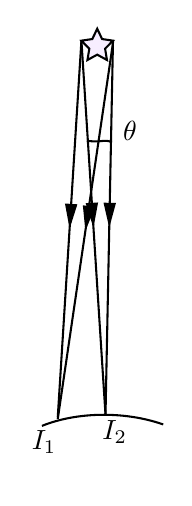
\begin{tikzpicture}[x=0.75pt,y=0.75pt,yscale=-1,xscale=1]
%uncomment if require: \path (0,300); %set diagram left start at 0, and has height of 300

%Shape: Star [id:dp7993730556190444] 
\draw  [fill={rgb, 255:red, 144; green, 19; blue, 254 }  ,fill opacity=0.07 ] (115,22.33) -- (117.35,27.3) -- (122.61,28.09) -- (118.8,31.95) -- (119.7,37.41) -- (115,34.83) -- (110.3,37.41) -- (111.2,31.95) -- (107.39,28.09) -- (112.65,27.3) -- cycle ;
%Straight Lines [id:da6010958544087177] 
\draw    (107.39,28.09) -- (119,208.33) ;
\draw [shift={(113.2,118.21)}, rotate = 266.31] [fill={rgb, 255:red, 0; green, 0; blue, 0 }  ][line width=0.08]  [draw opacity=0] (12,-3) -- (0,0) -- (12,3) -- cycle    ;
%Straight Lines [id:da5792212007108453] 
\draw    (122.61,28.09) -- (119,208.33) ;
\draw [shift={(120.8,118.21)}, rotate = 271.15] [fill={rgb, 255:red, 0; green, 0; blue, 0 }  ][line width=0.08]  [draw opacity=0] (12,-3) -- (0,0) -- (12,3) -- cycle    ;
%Shape: Arc [id:dp02266441256288565] 
\draw  [draw opacity=0] (88.36,213.69) .. controls (97.39,210.04) and (108.63,208.04) .. (120.75,208.37) .. controls (130.27,208.63) and (139.16,210.3) .. (146.81,213) -- (119.93,238.36) -- cycle ; \draw   (88.36,213.69) .. controls (97.39,210.04) and (108.63,208.04) .. (120.75,208.37) .. controls (130.27,208.63) and (139.16,210.3) .. (146.81,213) ;
%Curve Lines [id:da2800220853905422] 
\draw    (110,76.33) .. controls (118,77.33) and (118,75.33) .. (122,77) ;
%Straight Lines [id:da7563818948167416] 
\draw    (107.39,28.09) -- (96,209.33) ;
\draw [shift={(101.7,118.71)}, rotate = 273.6] [fill={rgb, 255:red, 0; green, 0; blue, 0 }  ][line width=0.08]  [draw opacity=0] (12,-3) -- (0,0) -- (12,3) -- cycle    ;
%Straight Lines [id:da6535572732710992] 
\draw    (122.61,29.09) -- (96,210.33) ;
\draw [shift={(109.3,119.71)}, rotate = 278.35] [fill={rgb, 255:red, 0; green, 0; blue, 0 }  ][line width=0.08]  [draw opacity=0] (12,-3) -- (0,0) -- (12,3) -- cycle    ;

% Text Node
\draw (126,65.4) node [anchor=north west][inner sep=0.75pt]    {$\theta $};
% Text Node
\draw (82,214.4) node [anchor=north west][inner sep=0.75pt]    {$I_{1}$};
% Text Node
\draw (116,209.4) node [anchor=north west][inner sep=0.75pt]    {$I_{2}$};


\end{tikzpicture}

    \caption{HBT实验测量天狼星的张角}
    \label{fig:hbt-initial-experiment}
\end{figure}

1954年两位电气工程师Robert Hanbury Brown%
\footnote{
    Hanbury Brown是一个复姓。
}%
和Richard Q. Twiss试图想出一种方法测量天狼星的张角。如\autoref{fig:hbt-initial-experiment}所示,我们在地球上安装两个相隔一定距离的探测器,用它们接受天狼星两端的光。
与通常的干涉实验不同,Hanbury Brown和Twiss测量\emph{二阶相干度}

这个说法——遥远星体上相隔很远的两点产生的光不知道怎么回事具有很好的相干性——不出意外地引起了轩然大波。

\subsubsection{经典电动力学解释}

\subsubsection{两个激光器产生的光束的干涉}

两个激光器产生的光似乎是相干的?

实际上激光器产生的是相干态光而不是光子数确定的多光子玻色波函数。

\subsubsection{玻色-爱因斯坦凝聚态中的干涉}

\chapter{线性过程}

我们这一节要做的事情和\autoref{chap:linear-matter-no-scattering}中没有什么本质上的区别:我们讨论线性过程——或者说没有光子生灭的过程。
对这样的一个过程,我们选择海森堡绘景,设$\{a_k\}$是某组模式,$\{b_l \}$是它经过一个线性过程演化之后的模式,即\begin{equation}
    b_l^\dagger = S_{lk} a^\dagger_k,
\end{equation}
且根据幺正性要求我们有
\begin{equation}
    a_k^\dagger = S_{kl}^* b^\dagger_l,
\end{equation}
则使用$a$算符表述的系统状态是
\begin{equation}
    \ket*{\psi}_\text{in} = f(\{ a_k^\dagger \}) \ket*{0},
\end{equation}
而使用$b$算符表述的系统状态是
\begin{equation}
    \ket*{\psi}_\text{out} = f(\{ S_{kl}^* b_l^\dagger \}) \ket*{0}.
\end{equation}
例如,对相干态我们有
\begin{equation}
    \ket*{\alpha} = 
\end{equation}
因此我们有
\begin{equation}
    \beta_l = S_{lk}^* \alpha_k ,
\end{equation}
即相干态的标签$\alpha$的时间演化方式和$a$算符完全一样,正好是预期的结果。

\section{分束器和反射镜}

\subsubsection{单光子变换矩阵}

\begin{figure}
    \centering
    

\tikzset{every picture/.style={line width=0.75pt}} %set default line width to 0.75pt        

\begin{tikzpicture}[x=0.75pt,y=0.75pt,yscale=-1,xscale=1]
%uncomment if require: \path (0,300); %set diagram left start at 0, and has height of 300

%Shape: Rectangle [id:dp18697858606449214] 
\draw   (153.4,128.89) -- (213.6,186.03) -- (199.6,200.77) -- (139.4,143.64) -- cycle ;
%Straight Lines [id:da46542740864676957] 
\draw    (93,164) -- (161,164) ;
\draw [shift={(127,164)}, rotate = 180] [fill={rgb, 255:red, 0; green, 0; blue, 0 }  ][line width=0.08]  [draw opacity=0] (12,-3) -- (0,0) -- (12,3) -- cycle    ;
%Straight Lines [id:da7146894444198257] 
\draw    (179,152) -- (247,152) ;
\draw [shift={(213,152)}, rotate = 180] [fill={rgb, 255:red, 0; green, 0; blue, 0 }  ][line width=0.08]  [draw opacity=0] (12,-3) -- (0,0) -- (12,3) -- cycle    ;
%Straight Lines [id:da09168332684614966] 
\draw    (161,164) -- (161,235.67) ;
\draw [shift={(161,199.83)}, rotate = 270] [fill={rgb, 255:red, 0; green, 0; blue, 0 }  ][line width=0.08]  [draw opacity=0] (12,-3) -- (0,0) -- (12,3) -- cycle    ;
%Straight Lines [id:da6638826474470239] 
\draw    (178,80.33) -- (178,152) ;
\draw [shift={(178,116.17)}, rotate = 270] [fill={rgb, 255:red, 0; green, 0; blue, 0 }  ][line width=0.08]  [draw opacity=0] (12,-3) -- (0,0) -- (12,3) -- cycle    ;

% Text Node
\draw (74,153.4) node [anchor=north west][inner sep=0.75pt]    {$\mathcal{E}_{1}$};
% Text Node
\draw (170,58.4) node [anchor=north west][inner sep=0.75pt]    {$\mathcal{E}_{2}$};
% Text Node
\draw (253,142.4) node [anchor=north west][inner sep=0.75pt]    {$\mathcal{E} '_{1}$};
% Text Node
\draw (152,238.4) node [anchor=north west][inner sep=0.75pt]    {$\mathcal{E} '_{2}$};


\end{tikzpicture}

    \caption{分束器}
    \label{fig:beam-splitter}
\end{figure}

一个分束器是一个形如\autoref{fig:beam-splitter}的装置,它将两束光变换为另外两束光。分束器的变换矩阵为
\begin{equation}
    \pmqty{\tilde{\mathcal{E}}_1 \\ \tilde{\mathcal{E}}_2} = \pmqty{t & r \\ - r^* & t} \pmqty{\mathcal{E}_1 \\ \mathcal{E}_2}.
\end{equation}
这里,$-r^*$的负号来自幺正性的要求;实际上这就是经典电动力学中的半波损失。
例如,我们有\SI{50}{\percent}分束器,其变换矩阵为
\begin{equation}
    S = \frac{1}{\sqrt{2}} \pmqty{1 & 1 \\ -1 & 1}.
\end{equation}

\subsection{Aspect实验}

要证明单光子具有量子性,最好的办法是使用一些这样的实验:它的一种版本能够证明光子的粒子性,它的另一个仅仅做了少许修正的版本(比如说探测器被移动到别的位置)能够证明光子的波动性。
两个版本区别很小这件事能够排除实验装置和光的复杂相互作用显著地改变了光的行为这样的说法,而粒子性和波动性同时出现则强烈暗示需要量子理论描述光。
1986年的Aspect实验是这种实验的一个典范。

\begin{equation}
    \begin{aligned}
        S &= \frac{1}{\sqrt{2}} \pmqty{1 & 1 \\ -1 & 1} \pmqty{ \dmat{\ee^{\ii \varphi / 2}, \ee^{- \ii \varphi / 2}} } \frac{1}{\sqrt{2}} \pmqty{1 & 1 \\ -1 & 1}  \\
        &= \pmqty{\cos\frac{\varphi}{2} & \sin\frac{\varphi}{2} \\ - \sin\frac{\varphi}{2} & \cos\frac{\varphi}{2}}.
    \end{aligned}
\end{equation}

\subsection{Zeilinger实验}

A.Zeilinger
一种更加简明的实验是这样的:同样使用分束器和反射镜,构造这样的光路:

\subsection{Hong-Ou-Mondel效应}



\subsection{条件量子态}

\begin{figure}
    \centering
    

\tikzset{every picture/.style={line width=0.75pt}} %set default line width to 0.75pt        

\begin{tikzpicture}[x=0.75pt,y=0.75pt,yscale=-1,xscale=1]
%uncomment if require: \path (0,300); %set diagram left start at 0, and has height of 300

%Shape: Rectangle [id:dp9242602312444221] 
\draw   (193,119) -- (263,119) -- (263,159) -- (193,159) -- cycle ;
%Straight Lines [id:da7075004076272056] 
\draw    (127,140) -- (193,140) ;
\draw [shift={(160,140)}, rotate = 180] [fill={rgb, 255:red, 0; green, 0; blue, 0 }  ][line width=0.08]  [draw opacity=0] (12,-3) -- (0,0) -- (12,3) -- cycle    ;
%Straight Lines [id:da42996678105947117] 
\draw    (263,140) -- (348,79) ;
\draw [shift={(305.5,109.5)}, rotate = 504.33] [fill={rgb, 255:red, 0; green, 0; blue, 0 }  ][line width=0.08]  [draw opacity=0] (12,-3) -- (0,0) -- (12,3) -- cycle    ;
%Straight Lines [id:da7812145894988733] 
\draw    (263,140) -- (348,201) ;
\draw [shift={(305.5,170.5)}, rotate = 215.67000000000002] [fill={rgb, 255:red, 0; green, 0; blue, 0 }  ][line width=0.08]  [draw opacity=0] (12,-3) -- (0,0) -- (12,3) -- cycle    ;
%Straight Lines [id:da29099064424770593] 
\draw    (348,201) -- (426,201) ;
\draw [shift={(387,201)}, rotate = 180] [fill={rgb, 255:red, 0; green, 0; blue, 0 }  ][line width=0.08]  [draw opacity=0] (12,-3) -- (0,0) -- (12,3) -- cycle    ;
%Shape: Chord [id:dp5153738151961664] 
\draw   (425.67,179) .. controls (438.92,179.02) and (449.76,188.55) .. (450,200.52) .. controls (450.23,212.67) and (439.46,222.73) .. (425.93,223) -- cycle ;
%Straight Lines [id:da7719196407492437] 
\draw  [dash pattern={on 4.5pt off 4.5pt}]  (450,201) -- (466,201) ;
%Straight Lines [id:da27041501657550526] 
\draw    (348,79) -- (460,79) ;
\draw [shift={(404,79)}, rotate = 180] [fill={rgb, 255:red, 0; green, 0; blue, 0 }  ][line width=0.08]  [draw opacity=0] (12,-3) -- (0,0) -- (12,3) -- cycle    ;
%Straight Lines [id:da20605124142789344] 
\draw  [dash pattern={on 4.5pt off 4.5pt}]  (466,105.33) -- (466,201) ;
%Shape: Rectangle [id:dp3038430486229844] 
\draw   (471,63) -- (459.92,63) -- (459.92,105.33) -- (471,105.33) -- cycle ;
%Straight Lines [id:da18864355508447694] 
\draw    (471,79) -- (526,79) ;
\draw [shift={(498.5,79)}, rotate = 180] [fill={rgb, 255:red, 0; green, 0; blue, 0 }  ][line width=0.08]  [draw opacity=0] (12,-3) -- (0,0) -- (12,3) -- cycle    ;

% Text Node
\draw (228,139) node   [align=left] {SHG};
% Text Node
\draw (118,115.4) node [anchor=north west][inner sep=0.75pt]    {$E_{\text{p}}$};
% Text Node
\draw (350,54.4) node [anchor=north west][inner sep=0.75pt]    {$E_{1}$};
% Text Node
\draw (346,177.4) node [anchor=north west][inner sep=0.75pt]    {$E_{2}$};


\end{tikzpicture}

    \caption{产生条件量子态的装置}
\end{figure}

考虑\autoref{sec:chi-2-wave}的量子版本,它会引入相互作用哈密顿量
\begin{equation}
    V = \int \dd[3]{\vb*{r}} \chi^{(2)} : \vb*{E}_\text{p}^\dagger \vb*{E}_1 \vb*{E}_2 + \text{h.c.},
\end{equation}
其中$\vb*{E}_\text{p}$为泵浦光。

\subsection{光量子计算}

条件量子态的产生让人产生一种想象:如果我们能够找到一个足够强的二阶非线性晶体,那么就能够实现\concept{单光子非线性性}:这意味着我们可以用一个光子控制另一个光子。
例如,就SHG过程而言,如果它足够强,使得两个不同模式的光子共同存在时就能够聚合为一个另一个模式的光子,那么这就是一个与门。

可惜的是目前在普通的非线性晶体中无法实现这种过程。冷原子体系能够产生强烈的光子-光子耦合。

\begin{figure}
    \centering
    

\tikzset{every picture/.style={line width=0.75pt}} %set default line width to 0.75pt        

\begin{tikzpicture}[x=0.75pt,y=0.75pt,yscale=-1,xscale=1]
%uncomment if require: \path (0,300); %set diagram left start at 0, and has height of 300

%Shape: Square [id:dp5812640844481787] 
\draw   (206,108) -- (232,108) -- (232,134) -- (206,134) -- cycle ;
%Straight Lines [id:da23406010312221892] 
\draw    (206,134) -- (232,108) ;

%Straight Lines [id:da12470247976338489] 
\draw    (105,121) -- (219,121) ;
\draw [shift={(162,121)}, rotate = 180] [fill={rgb, 255:red, 0; green, 0; blue, 0 }  ][line width=0.08]  [draw opacity=0] (12,-3) -- (0,0) -- (12,3) -- cycle    ;
%Straight Lines [id:da8231064877854108] 
\draw    (219,121) -- (333,121) ;
%Straight Lines [id:da03344738041998285] 
\draw    (219,121) -- (219,211.33) ;
\draw [shift={(219,166.17)}, rotate = 90] [fill={rgb, 255:red, 0; green, 0; blue, 0 }  ][line width=0.08]  [draw opacity=0] (12,-3) -- (0,0) -- (12,3) -- cycle    ;
%Straight Lines [id:da3041250062025471] 
\draw    (219,53.33) -- (219,121) ;
\draw [shift={(219,87.17)}, rotate = 90] [fill={rgb, 255:red, 0; green, 0; blue, 0 }  ][line width=0.08]  [draw opacity=0] (12,-3) -- (0,0) -- (12,3) -- cycle    ;
%Shape: Square [id:dp9371797224374869] 
\draw   (320,108) -- (346,108) -- (346,134) -- (320,134) -- cycle ;
%Straight Lines [id:da05948010816759908] 
\draw    (320,134) -- (346,108) ;

%Straight Lines [id:da4093214516440322] 
\draw    (333,121) -- (447,121) ;
\draw [shift={(390,121)}, rotate = 180] [fill={rgb, 255:red, 0; green, 0; blue, 0 }  ][line width=0.08]  [draw opacity=0] (12,-3) -- (0,0) -- (12,3) -- cycle    ;
%Straight Lines [id:da3614482552806686] 
\draw    (333,121) -- (333,211.33) ;
\draw [shift={(333,166.17)}, rotate = 90] [fill={rgb, 255:red, 0; green, 0; blue, 0 }  ][line width=0.08]  [draw opacity=0] (12,-3) -- (0,0) -- (12,3) -- cycle    ;
%Straight Lines [id:da7606039605325201] 
\draw    (333,53.33) -- (333,121) ;
\draw [shift={(333,87.17)}, rotate = 90] [fill={rgb, 255:red, 0; green, 0; blue, 0 }  ][line width=0.08]  [draw opacity=0] (12,-3) -- (0,0) -- (12,3) -- cycle    ;
%Straight Lines [id:da4133297014948891] 
\draw    (219,53.33) -- (274,53.33) ;
%Straight Lines [id:da6242316516385615] 
\draw    (333,53.33) -- (388,53.33) ;
%Shape: Chord [id:dp8695097730726187] 
\draw   (274.11,38.08) .. controls (283.31,38.1) and (290.82,44.7) .. (290.98,53) .. controls (291.14,61.42) and (283.68,68.4) .. (274.3,68.58) -- cycle ;
%Shape: Chord [id:dp8381933152038832] 
\draw   (388.11,38.08) .. controls (397.31,38.1) and (404.82,44.7) .. (404.98,53) .. controls (405.14,61.42) and (397.68,68.4) .. (388.3,68.58) -- cycle ;

% Text Node
\draw (14,98.4) node [anchor=north west][inner sep=0.75pt]    {$\alpha \ket{0} +\beta \ket{1} +\gamma \ket{2}$};
% Text Node
\draw (204,214.4) node [anchor=north west][inner sep=0.75pt]    {$\ket{1}$};
% Text Node
\draw (322,212.4) node [anchor=north west][inner sep=0.75pt]    {$\ket{0}$};


\end{tikzpicture}

    \caption{通过观察实现受控相位门}
\end{figure}

受控相位门
\begin{equation}
    \ket*{\psi_\text{c}'} = \alpha \ket*{0} + \beta \ket*{1} - \gamma \ket*{2}
\end{equation}
